\documentclass[a4paper]{article}
\usepackage{graphicx}
\usepackage[bookmarks=true]{hyperref}
\usepackage{bookmark}
\usepackage[margin=1.2in]{geometry}
\usepackage{float}
\usepackage{caption}
\usepackage{hyperref}
\usepackage[english]{babel}
\usepackage{graphicx}

\title{Functional Requirements}
\author{The Baobab Team}

\begin{document}

\newpage
\input{./TitlePage.tex}

\newpage
\begin{center}
\LARGE \textbf{Member details}\\
\begin{tabular}{ll}
Ephiphania Munava&10624610\\
Lutfiyya Razak&10198408\\
Lerato Molokomme&11197961\\
Mpedi Mello&11210754\\
Patience Mtsweni&11116774\\
Tsepo Ntsaba&10668544\\

\end{tabular}
\end{center}

\newpage
\tableofcontents
\listoffigures
\newpage

\section{\textbf{\huge{Introduction}}}
\subsection{Purpose}
The purpose of this project is to extend Linphone's Instant Messaging (IM) implementation on Android platforms to include group chat and to implement other minor improvements to Linphones IM capabilities and user interface. 

\subsection{Scope}
We are required to develop the following functionality for the Linphone project:
\begin{itemize}
\item Group chat (Invite additional members to a chat, all members receive chats)
\item Secure group chat (AES256)
\item Creation and deletion of groups
\item Voice record and send over IM
\item Improve the messaging user interface
	\begin{itemize}
		\item Spacing between words are terrible
		\item Make text bigger
		\item Blocks indents required to better specify who said what
		\item Presence indication to show a remote user is typing
		\item User picture portraits
	\end{itemize}
\end{itemize}

%Overview
\section{\textbf{\huge{Overview of Linphone Group Chat}}}
\large{Diagram to show an abstract overview of the Linphone Group Chat. This system will be discussed in greater detail in the rest of the article.}\\
\begin{figure}[H]
\centering
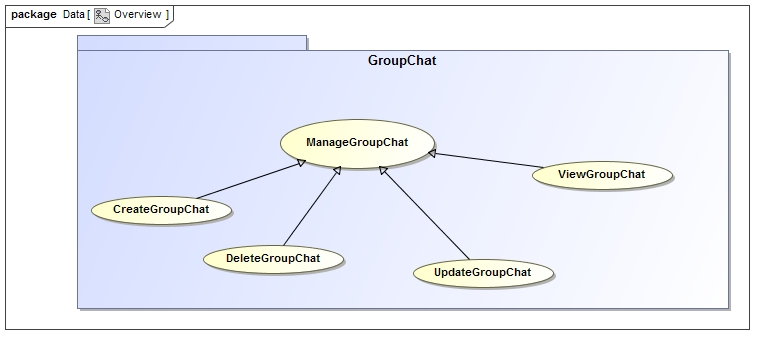
\includegraphics[width=1\linewidth]{./pictures/Overview.jpg}
\caption{Overview of Linphone group chat}
\end{figure}
\newpage


%Linphone group chat
\section{\textbf{\huge{Linphone Group Chat}}}

%CREATE GROUP CHAT
\subsection{Create Group Chat}
\subsubsection{Required Functionality:} 
\begin{figure}[H]
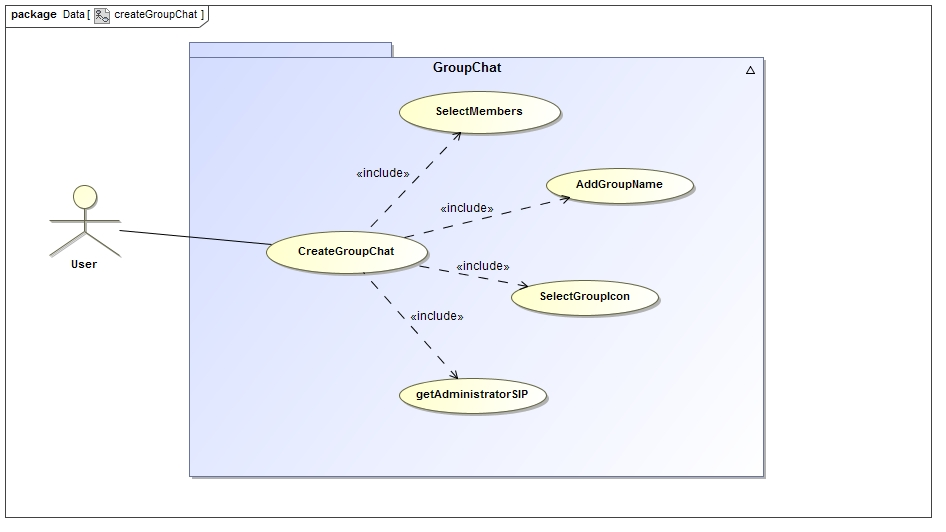
\includegraphics[width=1\linewidth]{./pictures/createGroupChat.jpg}
\caption{Create Group Chat use case diagram}
\end{figure}

\textbf{Description:}This use case encapsulates the ability for a user to create a new group chat that will be associated with a number of members. 
Each group chat will have a chat room to start with. The creator of the group chat will be the administrator with the ability to add new  members, as well as remove them, and also delete the group chat.

\subsubsection{Prioritization:}Critical
\subsubsection{Conditions and Data Structures:}
\textbf{Pre-Conditions:}
\begin{itemize}
	\item The user wanting to create a new group chat should have a sip address and have a linphone application. 
	\item The user should have the sip addresses for the members they want to add to the group.
\end{itemize}
\textbf{Post-Conditions:}
\begin{itemize}
	\item A message is displayed to inform the creator of the group chat that the creation has been successful. Users can now start chatting in the group.
	\item If this service has been rejected, an exception is thrown and an error message will be displayed to the user.
\end{itemize}
	
\subsubsection{Process Specifications:} 
\begin{figure}[H]
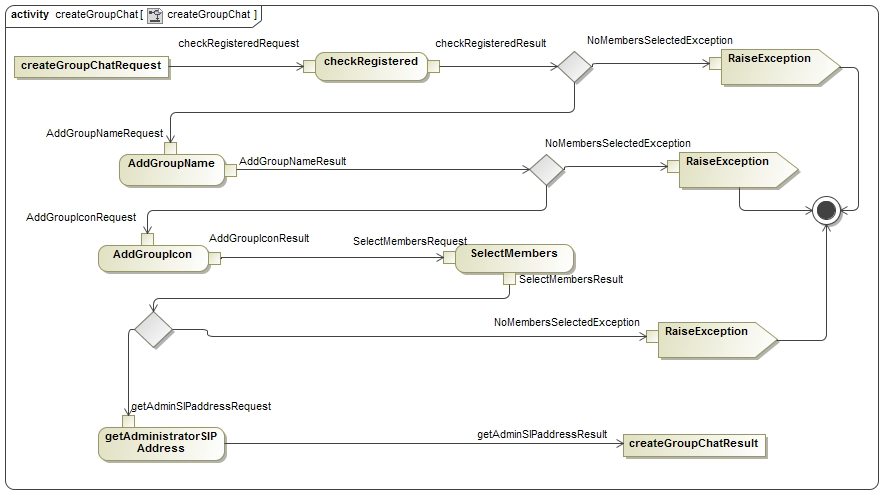
\includegraphics[width=1\linewidth]{./pictures/create_GroupChat.jpg}
\caption{Create Group Chat activity diagram }
\end{figure}


% View GROUP CHAT
\subsection{View Group Chat}

\subsubsection{Required Functionality:} 
\begin{figure}[H]
\includegraphics[width=1\linewidth]{./pictures/viewGroupChat.jpg}
\caption{View Group Chat use case diagram}
\end{figure}

\textbf{Description:}This use case includes the ability to View Group Chat, this is, to view the chats in the Group (and thus have access to them), and also to view the
properties of the specific group (i.e. the members of the group, date of creation and the creator of the group as well as chat history).

\subsubsection{Prioritization:} Critical

\subsubsection{Conditions and Data Structures:}
\textbf{Pre-Conditions:}
\begin{itemize}
	\item The user should be associated with the group. 
\end{itemize}
\textbf{Post-Conditions:}
\begin{itemize}
	\item User can view chat properties.
\end{itemize}

\subsubsection{Process Specifications:} 
\begin{figure}[H]
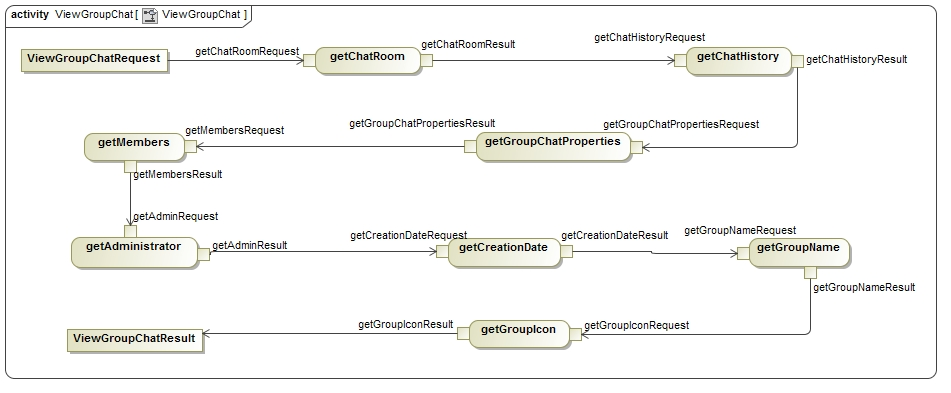
\includegraphics[width=1\linewidth]{./pictures/view_GroupChat.jpg}
\caption{View Group Chat activity diagram}
\end{figure}


%UPDATE GROUP CHAT
\subsection{Update Group Chat}
\subsubsection{Required Functionality:} 
\begin{figure}[H]
\includegraphics[width=1\linewidth]{./pictures/updateGroupChat.jpg}
\caption{Update Group Chat use case diagram}
\end{figure}

\subsection{Update Group Chat}
\textbf{Description:}This use case gives the ability for a user edit group icon, get members, update group chat, add members, remove members and edit group name. 

\subsubsection{Prioritization:} Important

\subsubsection{Conditions and Data Structures:}
\textbf{Pre-Conditions:}
\begin{itemize}
	\item The user should be associated with the group. 
\end{itemize}
\textbf{Post-Conditions:}
\begin{itemize}
	\item A message is displayed to let the user know that the update has been done successfully
	\item If the service was rejected, an exception is thrown and an error message is displayed to let the user know.
\end{itemize}

\subsubsection{Process Specifications:} 
\begin{figure}[H]
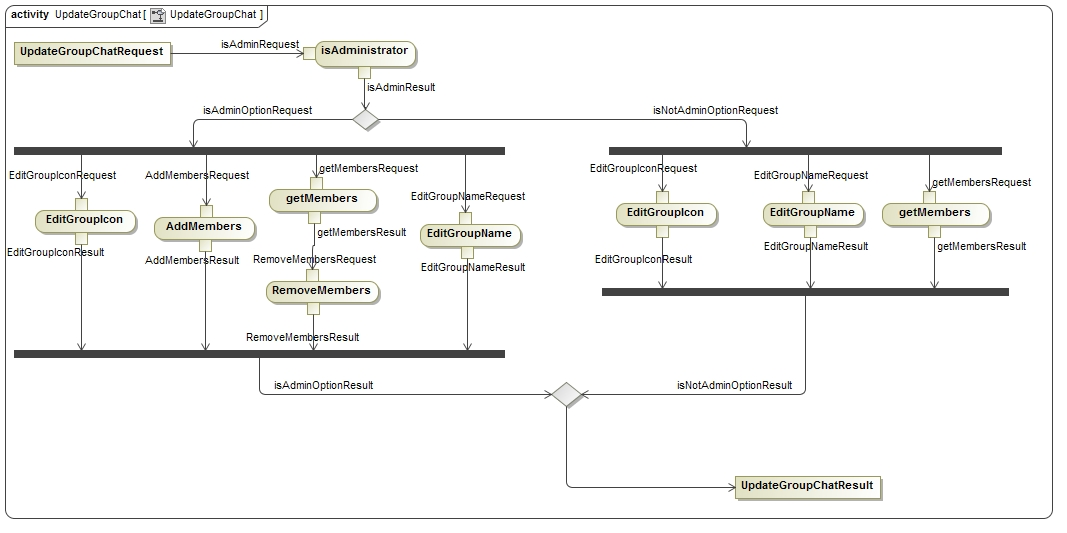
\includegraphics[width=1\linewidth]{./pictures/update_GroupChat.jpg}
\caption{Update Group Chat activity diagram}
\end{figure}



%DELETE GROUP CHAT
\subsection{Delete Group Chat}

\subsubsection{Required Functionality:}

\begin{figure}[H]
\includegraphics[width=1\linewidth]{./pictures/deleteGroupChat.jpg}
\caption{Delete Group Chat use case diagram}
\end{figure} 

\textbf{Description:}This use case includes the ability to delete a Group Chat when the creator of the group chats delete the group. Only the creator of the Group Chat will be able to delete a Group Chat, except if he removes himself from the group then a new group administrator will be assigned.

\subsubsection{Prioritization:} Critical

\subsubsection{Conditions and Data Structures:}
\textbf{Pre-Conditions:}
\begin{itemize}
	\item The user should be associated with the group. 
	\item The user should be the group creator. 
\end{itemize}
\textbf{Post-Conditions:}
\begin{itemize}
	\item The group chat is deleted and archived for future reference. 
\end{itemize}

\subsubsection{Process Specifications:} 
\begin{figure}[H]
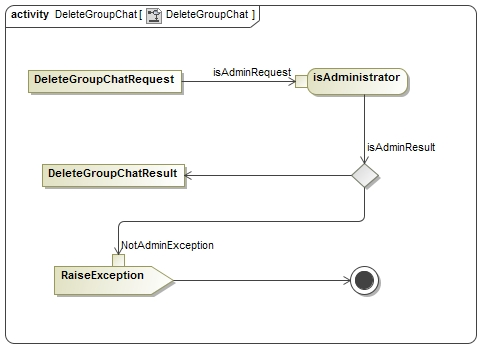
\includegraphics[width=1\linewidth]{./pictures/delete_GroupChat.jpg}
\caption{Delete Group Chat activity diagram}
\end{figure}

\subsection{Domain model}
This is the domain model for the group chat
\begin{figure}[H]
\centering
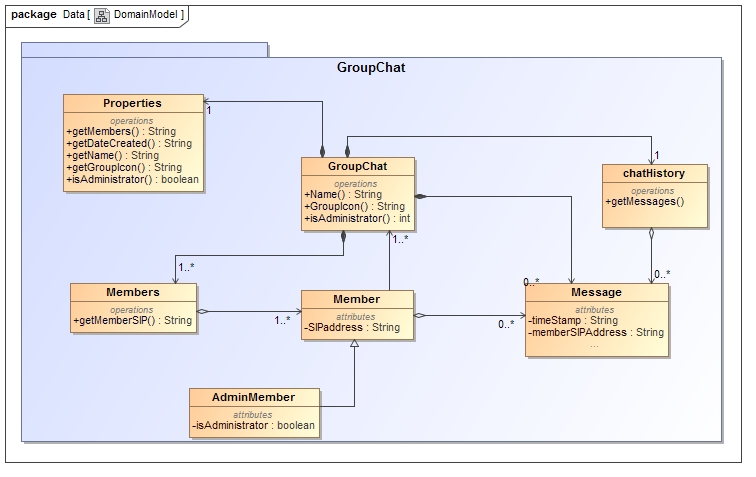
\includegraphics[width=1\linewidth]{./pictures/DomainModel.jpg}
\caption{Domain model for Group Chat}
\end{figure}

Note that the relationship between the GroupChat and Properties,Members, Message and chatHistory is a composite relationship because they are only accessible from the GroupChat and if the GroupChat is deleted, they all are also deleted.\\
\\
There is a aggregation relationship between Members and member because the members class has to consists of one or more members. \\
\\
There is also a specialization relationship between member and AdminMember because a member can be administrator member(can add members, remove members,delete group) or a basic group member(can edit group icon,group name and view members).
\end{document}